\chapter{Introduction}\label{ch:introduction}
Distributed sensor networks (DSNs) consist of any number of sensors that collect and sense information about the physical environment around them. The sensors that make up these networks can either be homogeneous or heterogeneous. Distributed sensor networks are dynamic in that sensors can be added or removed from the network at any time. DSNs also increasingly include mobile sensors as well. With the onset of the Internet of Things (IoT), it is easier than ever to build and deploy distributed sensor networks. Further, mobile devices, such as mobile phones, are seeing increased usage as intelligent sensing agents.

Distributed sensor network (DSN) optimization is a broad topic with many different facets to consider. Much of the literature on the topic focuses on optimizing data flow between sensors as data flows from sensor to sensor and eventually to a sink.

The focus of this dissertation however, is to deal with the challenges of a specific subset of DSNs. That subset is DSNs where data always flows directly from each sensor in the network to sink nodes where data is collected and analyzed, thus, eliminating the need to worry about intra-sensor communication, networking, and routing.

There are a broad range of technical challenges beyond the data sink. The introduction of the Internet of Things (IoT) has created an explosion of internet connected devices that sense a massive number of attributes about the physical world surrounding them. An increase in sensors has created an increase in multimodal data generation with the inverse problem of creating a decrease in the signal-to-noise ratio, making it more difficult to identify and classify signals of interest. Multimodal data provides challenges for analysis algorithms because each sensor may be streaming multiple physical features that need to be analyzed and dealt with independently and dependently. As the densities of sensors increase, analysis must be able to work with missing data, incorrect data, incomplete data, and data coming from a heterogeneous mix of hardware and sensor configurations. Further, we can no longer assume that sensors are static in time and location as mobile sensors are quickly becoming more prevalent, making analysis trickier. All of these issues require an increase in storage and computational resources. Therefore, we must find approaches to deal with sensor data to lessen these hurdles.

As DSNs scale, available storage must be balanced with the amount of data being retained. Further, once data is collected, we need strategies for turning sensor data into actionable data and insights. This generally involves detecting and classifying signals of interest. It's these last two important DSN challenges that are the focus of this dissertation.

\section{Converting Sensor Data into Actionable Insights}\label{sec:converting-sensor-data-into-actionable-insights}
Data collected from sensors is often a sampled payload of data points representing some feature in the physical world. As examples, weather stations produce sampled features relating to temperature, wind speed, and humidity, power meters produce a metric of total electricity consumed, power quality sensors produce sampled data points which include voltage, frequency, and THD, and infrasound networks produce sampled data which represent audio waveforms.

These features by themselves, while interesting, do not provide any context as to if there is a signal, what the signal is, when and where the signal came from, or what caused the signal in the first place. Detection and classification algorithms are used to attempt to extract some of these properties. Primitive data is aggregated and compared to other primitive data to find correlations in both time and space. Data is compared to historic data in an attempt to find patterns or other similarities. This type of data is more interesting in that we might learn more about a signal using these techniques, but they still don't provide actionable insights or causality information. Further, the problem of providing actionable insights is highly dependent on the sensing domain. Depending on other available sources of data, providing data fusion and context from outside of the DSN can be difficult.

Evaluation techniques for converting sensor data into actionable insights is provided in Section~\ref{subsec:evaluation-of-converting-primitive-data-into-actionable-insights}. Results of converting sensor data into actionable insights is provided in Section~\ref{sec:results-of-converting-primitie-data-into-actional-insights}.

\section{Big Data Management in DSNs}\label{sec:big-data-management-in-dsns}
Big Data is generally defined by the four V's; volume, velocity, variety, and value. These characteristics can be observed in many of the DSNs that exist and are being created today.

That is, distributed sensor networks create a large volume of data due to the abundance of IoT and mobile devices that make up DSNs. As communication infrastructures improve and hardware becomes smaller, smarter, and more energy efficient, sensors are able to send and transfer larger amounts of data. The ease of building and deploying sensors in DSNs means that more sensors can be produced much more cheaply allowing for more sensors to be used within a DSN, increasing coverage, but also increasing the volume of data.

Distributed sensor networks create a variety of data with different formats and data quality issues. Distributed sensor networks can produce data at high velocity. These characteristics of data produced from distributed sensor networks create a need for efficient architectures and specific algorithms designed for working with Big Data.

Further, sensor networks are often constrained in both computing power and available energy sources. This forces us to find comprises between data collection, onboard sensor processing, sensor communication, and network coordination.

As DSNs scale, the amount of data a DSN must store and process increases. At certain scales, DSNs simply can not store and process all of the primitive data that sensors are producing or process and store aggregate data products that detection and analysis routines produce. Designers of a DSN can either choose to collect and keep all data forever (from raw data to generated products), or they can implement strategies for systematically discarding (hopefully) non-interesting data. If the first option is chosen, then there is no risk of accidentally discarding signals of interest and data can be reanalyzed when analysis algorithms change or are tweaked. However, storage and analysis of such amounts of data can cause system degradation or even become unfeasible. If the second option is chosen, processes must be put in place that attempt to only store ``interesting" data and discard sensor noise.  The second option runs the risk of discarding important data and old data can not be reanalyzed under this approach. However, this approach provides the benefits of providing predictable data storage requirements that can be tuned and optimized for a particular domain and DSN.

Evaluation of big data management in DSNs is provided in Section~\ref{subsec:eval-big-data}. Results of big data management in DSNs is provided in Section~\ref{sec:dsn-system-requirements}.

\section{Traditional Approaches to DSN Optimization}\label{sec:traditional-approaches-to-dsn-optimization}
Much of the literature focuses on the reduction of bandwidth and communication between sensors nodes and between sensor nodes and the sink. This is mainly performed to manage sensor energy requirements allowing sensing to stay online longer or focus their energy usage for sensing or edge level computing. Anastasi et al\cite{anastasi_energy_2009} provide a literature review on techniques for energy conservation in wireless sensor networks. Many of these approaches utilize optimized triggering\cite{alippi_adaptive_2010} or exploitation of topology knowledge\cite{warrier2007much} to minimize sensor communications and save sensor energy.  General approaches to Big Data management include compression\cite{tang2004compression} or storage systems where the goal is to have a distributed file system and move data close to where it is being processed, such as the Hadoop Distributed File System\cite{warrier2007much}. Other systems such as NiFi\cite{hughes2016survey} provide an interface for ingestion and movement of data between Big Data tools while also providing data provenance, but do not address data reduction and graceful degradation. Carney et al.\cite{carney2002monitoring} discuss how monitoring applications require management and clean up of stale sensor data. Much of the literature on topology management is written to decrease sensor energy requirements by exploiting the density of sensors within a sensing field topology. For example, the ASCENT\cite{cerpa2004ascent} framework provides adaptive self configuring sensors that exploit topology denseness to decrease sensor energy usage. Several other frameworks have been designed with the same goal of reducing energy usage by exploiting topology\cite{schurgers2002stem,schurgers2002topology}.

\section{Laha: An Abstract Framework for Adaptively Optimizing DSNs}\label{sec:laha:-an-abstract-framework-for-adaptively-optimizing-dsns}
In this dissertation, I describe an abstract distributed sensor network framework, Laha\footnote{Laha is a Hawaiian word meaning ``to distribute".}, that adaptively optimizes data storage using a tiered TTL approach and provides a mechanism in which typed aggregated data is continually refined to the point of being of becoming actionable.

The Laha data model can be conceptualized as a multilevel hierarchy which can be represented as a pyramid (see Figure~\ref{laha-abstract-overview}). Laha Actors act on the data model to move data upward through the levels and to apply optimizations downward through the levels. Many of these optimization techniques were developed independently. Laha provides a conceptual framework that enables them to work together.

The lowest level of the hierarchy stores all recently received raw sensor data. This data expires and is automatically removed within a limited period of time (for example, 1 hour) unless the data is found to be interesting, and is thus propagated upwards to the next level of the hierarchy.  Higher levels of the data hierarchy organize data in the same way, however each level adds context to the examined signal or signals. Context includes classifications, locality metrics, temporal metrics, or similarities to current or prior signals of interest. The highest level of the hierarchy, Phenomena, represents predictive capabilities of the sensor network which are then used to optimize and tune the lower levels. Phenomena also form the basis for providing actionable insights.

A high level summary of the Laha abstract framework is provided as Figure~\ref{laha-abstract-overview} which shows the levels and names of the hierarchy, a brief description of the functions of each level, and Laha's Actors and how they move data upwards (right hand side) and how they apply optimizations downwards (left hand side).

\begin{figure}
	\caption{Laha Conceptual Model Summary}
	\centering
	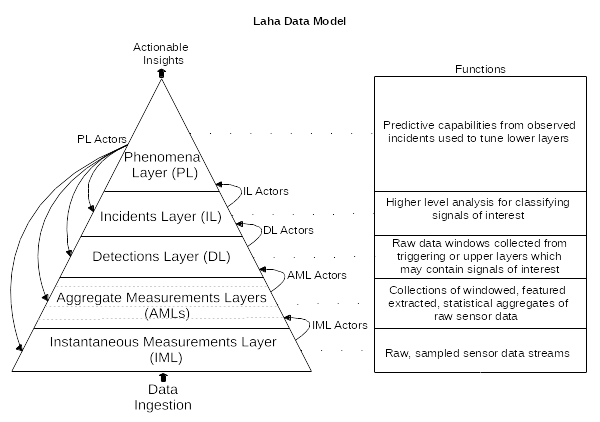
\includegraphics{figures/laha_abstract_overview.png}
	\label{laha-abstract-overview}
\end{figure}

The Laha framework provides two important benefits to DSNs:

\begin{enumerate}
	\item Converts sensor data into actionable data and insights
	\item Provides graceful degradation and metrics on storage requirements for voluminous sensor data
\end{enumerate}

Although not the main focus of this dissertation, Laha provides several tangential benefits with respect to the following DSN problem domains:

\begin{enumerate}
	\item Triggering optimizations
	\item Detection and classification optimizations
	\item Topological optimizations
	\item Sensor energy requirement optimizations
\end{enumerate}

These tangential benefits are provided by Laha Actors that exist within each level of the Laha framework. I don't claim that these techniques are novel, but I do claim that either all or a subset of these techniques are required to enable progress towards the main goals of this framework. To that end, Laha Actors implement several state of the art algorithms present in the literature that address these tertiary problems.

Laha was evaluated by designing and implementing two Laha-compliant reference implementations, OPQ and Lokahi. Open Power Quality (OPQ) is a power quality (PQ) network consisting of custom hardware and distributed software services that detect distributed PQ signals such as voltage sags and swells, frequency sags and swells, transients, THD, and other known PQ issues. OPQ Mauka is a distributed, plugin based middleware component of OPQ that performs higher level analysis, data management, and optimizations of the OPQ services. Lokahi is a distributed infrasound network consisting of mobile iOS and Android devices and multiple cloud based software services whose purpose is to supplement the International Monitoring System (IMS) in detecting large infrasound signals.

The reference implementations were designed and  deployed to test sites at UH Manoa and at the Infrasound Laboratory in Kailua-Kona, Big Island and abroad.

Data collected from the PQ network was validated against calibrated reference sensors that have already been installed at the power mains of a subset of buildings on campus. The Office of Energy Management at UH Manoa has given us full access to live and historic PQ data collected at these reference sensors. OPQ Boxes were co-located and placed in buildings with the reference sensors so that I could validate that the triggering and raw data streams I receive from the OPQ Boxes are in agreement with what the reference sensors are observing.

Data collected from the infrasound network was also validated against industry standard calibrated B\&K infrasound sensors. Further, signals in the infrasound network are known a priori since I am able to control the signals that are generated from our calibrated infrasound source, allowing further validation of received signals.

In order to evaluate the generality of the Laha framework, two separate Laha-compliant DSNs sensing different domains were designed, distributed, and evaluated.

The first Laha-compliant DSN is Open Power Quality (OPQ), a distributed DSN that collects and analyzes power quality (PQ) signals. PQ is a measure of the ``goodness" of the power feeding your electronics. The features that this network collects includes Voltage, Frequency, and THD. From these features, OPQ can classify the following PQ signals: Voltage dips/swells, Frequency dips/swells, high levels of THD, and transients. Another goal of this network is to detect distributed PQ signals. That is, the same signal detected on multiple sensors enables one to study how PQ signals move through a power grid. This network provided metrics on the number of incidents classified as well as numbers of correct predictions from Phenomena. The number of classified incidents are compared to industry standard PQ monitors co-located with OPQ sensors as a means of evaluating if Laha is capable of supporting the goals of this network.

The second Laha-compliant DSN is Lokahi, a distributed, mobile infrasound detection network. Infrasound consists of sounds waves that are less than 20 Hz. These signals are generated by large movements of the atmosphere and can be observed from large distances. Examples of infrasound sources include volcano eruptions, meteors, missile launches, and large explosions. In this network, Android and iOS devices were deployed with a special app that is capable of collecting acoustic signals as they travel through the atmosphere. As part of the evaluation, in this network, we collected and discriminated infrasound signals from different types of infrasound sources. Many of these signals are correlated with industry standard infrasound sensors to show that Laha is capable of supporting the infrasound detection goals of this network.

In order to evaluate the multi-level representation of the Laha Framework in the context of providing actionable data, I examined cyclical and predictable signals and tested whether or not Laha is able to utilize predictive analytics to provide actionable insights. To test this, I provided a number of false positive and false negatives for predictive analytic results. I evaluated if the sensing domain has any effect on how well Laha is able to provide actionable insights. I also claim that each level in the Laha-hierarchy is important in the process of deriving these insights. I provided data that either supports or opposes the usefulness of each level, whether the current number of levels is adequate, and whether the idea of using levels to provide actionable insights is useful at all.

I evaluated my claim that a tiered TTL approach to sensor data management provides the benefits of providing an configurable upper bounds on storage requirements for each Laha level, graceful degradation, and a reduction of sensor noise being stored. To test this, I implemented procedures for calculating storage bounds and determined if these theoretical bounds are valid in practice. Since it's possible that the TTL approach could throw away important data, I measured the number of false positives using the TTL approach as a means of evaluating its usefulness with a discussion of how detrimental these false positives might actually be to understanding and creating actionable data sets.

Finally, I evaluated multiple state of the art algorithms current in the literature for optimizing triggering, detection, classification, sensor energy usage, and topological modeling and provide metrics to their usefulness for making progress towards the larger goals of providing a generally useful representation for DSNs, converting primitive sensor data into actionable insights, and providing a tiered approach to DSN data management and storage requirements. I provided a discussion on whether these techniques are useful within the two domains that they are implemented, and if they are, how they contributed to the overall goals of this framework. I also show which combinations of tertiary techniques provide the most traction in solving the overall goals of this framework.

\section{Claims of Laha Abstract Framework}\label{sec:anticipated-contributions-of-laha}

\begin{tcolorbox}
The major claim of this dissertation is that the Laha Framework provides a generally useful representation of an abstract framework for real-time high-volume DSNs. I provide four related claims with design, evaluation, and results for each claim.
\end{tcolorbox}

\subsection{Generality of the Laha Framework}\label{subsec:generality-of-the-laha-framework}
The generality of the framework examines the ability for Laha to be a useful abstract framework in different domains while still meeting the requirements of those domains. This dissertation examines two domains, distributed power quality monitoring through the Open Power Quality network and distributed infrasound monitoring through the Lokahi Network.

To evaluate the generality of the network, I designed, implemented, and deployed two Laha-compliant reference networks in two different domains, power quality and infrasound. The design of these networks is described in Chapter~\ref{ch:system-design}. These reference implementations generate evidence for the ways in which Laha supports the goals of the sensor networks and ways in which it falls short. The evaluation of the generality of Laha is provided in the Evaluation chapter in Section~\ref{sec:use-laha-deployments-to-evaluate-the-main-goals-of-the-framework}. Results showing the generality of Laha are provided in the Results chapter in Section~\ref{sec:results-of-generality-of-this-framework}. The implementations also provide insights into the types of distributed sensor networks for which Laha is well-suited, and the types for which it is not. These insights are discussed in Section~\ref{subsec:discussion-on-types-of-dsns-laha-is-suitable-for}.

\subsection{Ability to Convert Primitive Data into Actionable Insights}\label{subsec:ability-to-convert-primitive-data-into-actional-insights}
Laha uses a tiered hierarchy to convert primitive data into actionable insights. As data passes ``upward" through the levels, context is applied to the data allowing different types of analysis to be performed on the data and more accurate conclusions to be drawn from the data.

The reference implementations enabled me to evaluate the multi-level representation system of tiered levels as described in the Evaluation Section~\ref{subsec:evaluation-of-converting-primitive-data-into-actionable-insights}. I claim that Laha enables a distributed sensor network to derive actionable insights from low level data, and that each of the levels is important to that process. The two reference implementations provide concrete data as to the set of levels that are useful in practice, or whether different levels would be more appropriate, or if the level strategy itself has problematic features. These results are provided in Sections~\ref{sec:results-of-converting-primitie-data-into-actional-insights} and~\ref{subsec:discussion-of-laha-levels}.

\subsection{Tiered Big Data Management}\label{subsec:tiered-big-data-management}
Laha additionally uses the tiered hierarchy to provide management of ``big data" relating to sensor acquisition and analysis. This is accomplished by providing a Time-to-Live (TTL) value for data that determines when that data should be garbage collected. I show how this approach is able to throw away noisy data while still identifying signals of interest.

I claim that a benefit of Laha's mechanism for managing data is that it enables the calculation of upper bounds on data storage requirements given the state of the network. I developed the analytical procedures required for calculating data storage requirements (as discussed in the Evaluation section~\ref{subsec:eval-big-data}), and determined if these procedures are valid in practice as shown in the Results Section~\ref{sec:dsn-system-requirements}. One obvious problem with a TTL approach is the possibility of false negatives: data that is discarded before it has been recognized as important. To quantify my results, I provide a comparison to ground truth sensors as described in the Evaluation Section~\ref{sec:validate-data-collected-by-laha-deployment} and shown in the Results Section~\ref{sec:ground-truth-analysis}.

\subsection{Tertiary Goals and Claims}\label{subsec:tertiary-goals-and-claims}
Finally, I assessed the ability to solve the tertiary problems of optimizing triggering, detection, classification, bandwidth, predictive analytics, and the ability to build a model of the sensing field. I claim that these problems need to be addressed in some form in order to solve the larger problems of turning primitive data into actionable insights and to provide a mechanism for managing large amounts of sensor data. I compare and contrast state of the art algorithms present in the literature to determine if they are effective in practice and useful for addressing the two larger problems. My evaluation in section~\ref{sec:evaluation-of-tertiary-goals} describe metrics required for demonstrating effectiveness. The results of the tertiary goals are provided in the Results Section~\ref{sec:results-of-tertiary-goals}.

\section{Contributions of Laha}\label{subsec:anticipated-contributions}
I have provided the following four contributions to the areas of DSNs, specifically regarding the problems of optimization and management of DSNs.

First, the Laha design, a novel abstract distributed sensor network that provides two useful properties relating to data management, converting primitive data to actionable data and tiered management of Big Data (Design~\ref{ch:system-design}, Evaluation~\ref{subsec:evaluation-of-converting-primitive-data-into-actionable-insights}, \ref{subsec:eval-big-data}, Results~\ref{sec:results-of-converting-primitie-data-into-actional-insights}, \ref{sec:dsn-system-requirements}).

Second, an evaluation of the Laha abstract framework through the deployment of two Laha-compliant reference implementations, validated data collection, and several experiments that are used to either confirm or deny the benefits claimed by Laha (Evaluation~\ref{sec:validate-data-collected-by-laha-deployment}, Results~\ref{sec:ground-truth-analysis}).

Third, two Laha-compliant reference implementations, OPQ and Lokahi, which can be used to form DSNs for the collection of distributed power quality signals and the distributed collection of infrasound signals. (Design~\ref{ch:system-design}, Evaluation~\ref{sec:deploy-laha-reference-implementations-on-test-sites}, \ref{subsec:evaluation-of-the-generality-of-this-framework}, Results~\ref{sec:results-of-generality-of-this-framework})

Fourth, a set of implications for modern distributed sensor networks as a result of the evaluation of Laha. That is, how does the confirmation or denial of Laha's benefits affect the field of modern DSNs moving forward? Results for these contributions can be found in Sections~\ref{subsec:discussion-on-types-of-dsns-laha-is-suitable-for} and ~\ref{subsec:discussion-of-laha-levels}.

\section{Organization of this Dissertation}\label{subsec:organization-of-this-dissertation}

Chapter~\ref{ch:introduction} introduces the the problem statements (Sections~\ref{sec:converting-sensor-data-into-actionable-insights} and~\ref{sec:big-data-management-in-dsns}), major components of the Laha abstract framework (Section~\ref{sec:laha:-an-abstract-framework-for-adaptively-optimizing-dsns}), traditional approaches to DSN optimization (Section \ref{sec:traditional-approaches-to-dsn-optimization}), contributions to the field of DSNs (Section~\ref{subsec:anticipated-contributions}), and major claims (Section \ref{sec:anticipated-contributions-of-laha}).

Chapter~\ref{ch:related-work} provides a literature review. Section~\ref{sec:big-data-and-distributed-sensor-networks} examines the literature on Big Data and DSNs. Literature on data management related to DSNs is provided in Section~\ref{sec:distributed-sensor-networks-and-big-data-management}. Section~\ref{sec:distributed-sensor-networks-and-predictive-analytics-and-forecasting} discusses literature on predictive analytics and forecasting. Section~\ref{sec:determining-topology-and-localization} examines literature on topology and localization. Section~\ref{sec:optimizations-for-triggering} discusses literature for optimizations for triggering.

Chapter~\ref{ch:system-design} outlines the Laha system design. Section~\ref{sec:big-data-management} provides the design of Big Data management. Section~\ref{sec:phenomena} examines the design of Phenomena. Section~\ref{sec:laha-actors:-acting-on-the-laha-data-model} provides the design of Laha Actors. Section~\ref{sec:opq:-a-laha-compliant-power-quality-dsn} discusses the design of the OPQ network. Finally, Section~\ref{sec:lokahi:-a-laha-compliant-infrasound-dsn} describes the design of the Lokahi network.

Chapter~\ref{ch:evaluation} provides an evaluation of Laha. Section~\ref{sec:deploy-laha-reference-implementations-on-test-sites} examines the deployments for the OPQ and Lokahi networks. Section~\ref{sec:validate-data-collected-by-laha-deployment} discusses evaluation techniques for data validation. Section~\ref{sec:use-laha-deployments-to-evaluate-the-main-goals-of-the-framework} examines strategies for evaluating the main goals of Laha. Section~\ref{sec:evaluation-of-tertiary-goals} provides the evaluation of tertiary goals.

Finally, Chapter~\ref{ch:results} provides results and discussions of results. Section~\ref{sec:ground-truth-analysis} provides results of data validation. Section~\ref{sec:results-of-generality-of-this-framework} discusses results for the generality of the Laha framework. Section~\ref{sec:results-of-converting-primitie-data-into-actional-insights} provides results detailing the conversion of primitive data into actionable insights. Section~\ref{sec:dsn-system-requirements} provides results for tiered management of Big Data. Section~\ref{sec:results-of-tertiary-goals} provides results of Laha's tertiary goals.

Chapter~\ref{ch:conclusion} provides concluding remarks and future directions. Section~\ref{sec:future-directions} outlines future directions. Future directions includes utilizing machine learning to improve triggering, detection, classification, and Phenomena, experimenting with window sizes and thresholds used in detection and classification algorithms, modifications to the Laha level hierarchy, data fusion, more complete simulations, metric collection, and the deployment of larger distributed sensor networks.









